\documentclass[12pt]{article}

\usepackage{amsmath}
\usepackage{amssymb}
\usepackage{amsfonts}
\usepackage{graphicx}
\usepackage{setspace}
\usepackage{geometry}
\usepackage{booktabs}
\usepackage{array}
\usepackage{hyperref}
\usepackage{float}
\usepackage{listings}
\usepackage{xcolor}
\usepackage[expansion=false]{microtype}

\geometry{margin=1in}
\setstretch{1.2}

\lstdefinestyle{python}{
    language=Python,
    basicstyle=\ttfamily\small,
    keywordstyle=\color{blue!70!black}\bfseries,
    stringstyle=\color{orange!80!black},
    commentstyle=\color{gray}\itshape,
    numbers=left,
    numberstyle=\tiny\color{gray},
    numbersep=8pt,
    frame=single,
    rulecolor=\color{gray!40},
    breaklines=true,
    showstringspaces=false,
    tabsize=4,
}

\title{Orbit Mania: A Newtonian Orbital Simulation and Reinforcement Learning Environment}

\author{
Adriel I. Santoso \\
Department of Mechanical and Aerospace Engineering \\
Tohoku University
}

\date{\today}

\begin{document}

\maketitle

\begin{abstract}
    \textit{Orbit Mania} is a dual-purpose software artifact combining a physics-accurate simulation of Keplerian orbital dynamics with a reinforcement learning (RL) environment conforming to the OpenAI Gymnasium standard. The simulation models spacecraft motion using polar-coordinate kinematics and a stylised Hohmann transfer mechanic. An autonomous agent trained via Proximal Policy Optimisation (PPO) navigates the same asteroid-evasion task presented to human players, enabling direct comparison of human and machine performance under resource constraints. This report describes the theoretical foundations, system architecture, simulation engine, RL environment specification, and training procedure.
\end{abstract}

% =============================================================
\section{Introduction}

\textit{Orbit Mania} is a project at the intersection of arcade game design, classical orbital mechanics, and machine learning. Originally conceived as a simple Pygame game in which a spacecraft evades asteroids while managing fuel, it has been substantially elevated into a dual-purpose artifact: a \textbf{physics-accurate simulation} of Keplerian orbital dynamics and a \textbf{reinforcement learning (RL) environment} conforming to the OpenAI Gymnasium standard.

The project pursues two complementary scientific goals:
\begin{enumerate}
    \item To model orbital motion using polar-coordinate kinematics and smooth radius interpolation, producing physically intuitive spacecraft behaviour.
    \item To train an autonomous agent using the Proximal Policy Optimisation (PPO) algorithm to survive the asteroid field, providing a benchmark for comparing human and machine decision-making under time pressure and resource constraints.
\end{enumerate}

The concept was motivated by the \textbf{Hohmann transfer}---a space manoeuvre encountered in the study of orbital mechanics that enables energy-efficient transitions between circular orbits. This transfer serves as the principal mechanic by which both human players and the AI agent switch between the two discrete orbital radii available in the environment.

% =============================================================
\section{Theoretical Background}

\subsection{Polar Representation of Circular Orbits}

The spacecraft's position is computed at each simulation tick using a polar-to-Cartesian transformation. The position vector $\mathbf{p}$ is given by

\begin{equation}
    \mathbf{p}(\theta) = \begin{bmatrix} r\cos\theta \\ r\sin\theta \end{bmatrix}
\end{equation}

where $r$ is the instantaneous orbital radius and $\theta$ is the current angular position, incremented each frame by a fixed angular speed $\dot\theta = 0.8$ degrees per tick.

\subsection{Circular Orbital Speed}

A stable circular orbit occurs when gravitational attraction exactly balances centripetal acceleration:
\begin{equation}
    \frac{GMm}{r^2} = \frac{mv^2}{r} \quad\Longrightarrow\quad v = \sqrt{\frac{GM}{r}}
\end{equation}

In the simulation the product $GM$ is a dimensionless constant tuned to give visually plausible motion ($GM = 1000$). The two available orbital radii are $r_1 = 125\,\text{px}$ (inner) and $r_2 = 225\,\text{px}$ (outer), yielding circular speeds of approximately $v_1 \approx 2.83\,\text{px/tick}$ and $v_2 \approx 2.11\,\text{px/tick}$ respectively.

\subsection{The Hohmann Transfer}

The Hohmann transfer is an orbital manoeuvre that transitions a spacecraft between two coplanar circular orbits using exactly two engine burns. The first burn accelerates the craft into an elliptical transfer orbit whose periapsis lies on the inner orbit and apoapsis on the outer; the second burn circularises the trajectory at the target radius.

In the game, this transfer is stylised: pressing \textsc{Space} sets a \textit{target radius} that the current radius interpolates towards at a fixed rate of 0.44 px/tick, producing the characteristic smooth spiral animation. This approximation preserves the qualitative character of the Hohmann transfer without requiring a full Keplerian elliptic integration.

\subsection{Reinforcement Learning}

Reinforcement learning frames interaction as an agent--environment loop. At each discrete time step $t$, the environment exposes a \textbf{state observation} $s_t \in \mathcal{S}$ to the agent. The agent selects an \textbf{action} $a_t \in \mathcal{A}$ according to its policy $\pi(a_t \mid s_t)$, and receives a scalar \textbf{reward} $r_t$ from the environment. The agent's objective is to maximise the expected discounted return:
\begin{equation}
    G_t = \sum_{k=0}^{\infty} \gamma^k r_{t+k}
\end{equation}
where $\gamma \in [0, 1)$ is a discount factor.

\subsubsection*{Proximal Policy Optimisation}

PPO \cite{schulman2017proximal} is a policy-gradient algorithm that alternates between sampling trajectories from the current policy and performing multiple stochastic gradient-ascent steps on a clipped surrogate objective:
\begin{equation}
    \mathcal{L}^{\text{CLIP}}(\theta) = \mathbb{E}_t\!\left[\min\!\left(
        r_t(\theta)\hat{A}_t,\;
        \text{clip}\!\left(r_t(\theta), 1-\varepsilon, 1+\varepsilon\right)\hat{A}_t
        \right)\right]
\end{equation}
where $r_t(\theta) = \pi_\theta(a_t|s_t)/\pi_{\theta_{\text{old}}}(a_t|s_t)$ is the probability ratio and $\hat{A}_t$ is a generalised advantage estimate. The clipping mechanism prevents excessively large policy updates, ensuring stable learning.

% =============================================================
\section{System Architecture}

The project is organised into four Python source files, each with a distinct responsibility, shown in Figure~\ref{fig:arch}.

\begin{figure}[h]
    \centering
    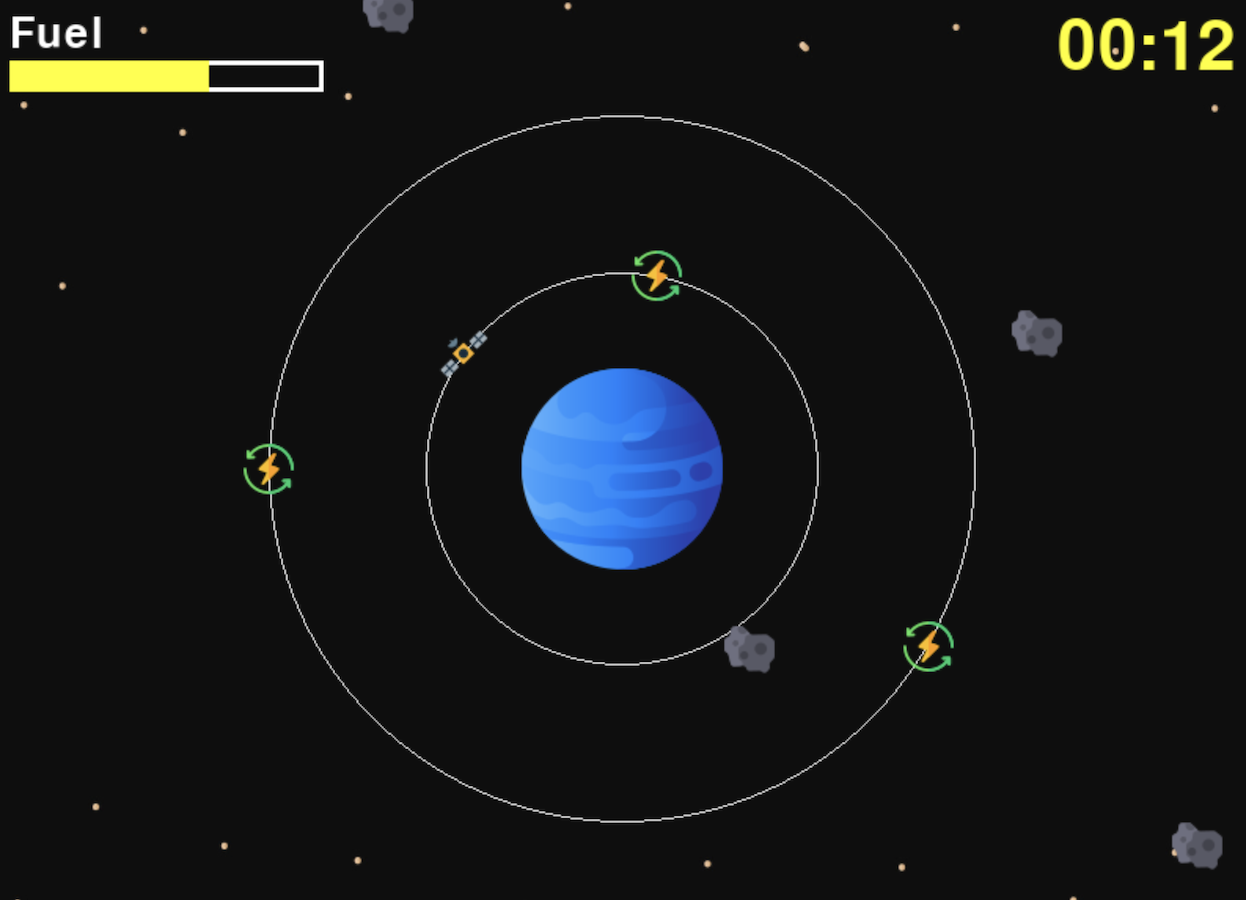
\includegraphics[scale=0.5]{../figures/figure1.png}
    \caption{In-game screenshot showing the spacecraft on the inner orbit, energy packets on both orbits, and incoming asteroids.}
    \label{fig:arch}
\end{figure}

\begin{center}
    \renewcommand{\arraystretch}{1.4}
    \begin{tabular}{>{\ttfamily}l p{9.5cm}}
        \toprule
        \textbf{File} & \textbf{Responsibility}                                       \\
        \midrule
        env.py        & Core simulation logic and Gymnasium interface. No graphics.   \\
        play.py       & Pygame rendering loop; bridges \texttt{env.py} to the screen. \\
        train.py      & Headless PPO training pipeline using Stable-Baselines3.       \\
        utilities.py  & Asset loader (sprites, sounds, fonts) for Pygame.             \\
        \bottomrule
    \end{tabular}
\end{center}

The critical design principle is \textbf{decoupling}: \texttt{env.py} runs with no graphical dependency. This allows \texttt{train.py} to spin up thousands of simulation ticks per second (CPU-bound only), accumulating experience far faster than real-time rendering would permit.

% =============================================================
\section{The Simulation Engine}

\subsection{State Variables}

Each episode maintains the following state:

\begin{itemize}
    \item $\theta$ (\texttt{angle}): current angular position in degrees, incremented each tick.
    \item $r$ (\texttt{radius}): instantaneous orbital radius in pixels.
    \item $r^*$ (\texttt{target\_radius}): target radius; either $r_1 = 125$ or $r_2 = 225$.
    \item $f$ (\texttt{fuel}): scalar in $[0, 100]$ representing energy reserves.
    \item $\sigma$ (\texttt{shield\_active}): Boolean; whether the deflector shield is active.
    \item $\mathcal{O}$: list of active obstacle dictionaries (position, velocity, radius).
    \item $\mathcal{E}$: list of active energy-packet dictionaries (position, radius).
\end{itemize}

\subsection{Simulation Tick}

Each call to \texttt{step(action)} performs the following operations in order:

\begin{enumerate}
    \item \textbf{Orbit switch}: if \texttt{action[0] = 1} and the ship is settled ($|r - r^*| < 1$), toggle $r^*$.
    \item \textbf{Radius lerp}: move $r$ towards $r^*$ by at most $\Delta r = 0.44$ px.
    \item \textbf{Angle advance}: $\theta \leftarrow \theta + 0.8°$.
    \item \textbf{Position update}: $\mathbf{p} = (r\cos\theta,\; r\sin\theta)$.
    \item \textbf{Fuel drain}: $f \leftarrow f - d$, where $d = 0.2$ (shield on) or $0.05$ (off).
    \item \textbf{Obstacle spawn}: spawn at scheduled interval (difficulty-dependent).
    \item \textbf{Energy packet spawn}: spawn if $|\mathcal{E}| < 5$ and interval elapsed.
    \item \textbf{Obstacle movement}: each obstacle translates leftward at its fixed speed.
    \item \textbf{Culling}: remove obstacles whose $x$-coordinate falls below $-1000$.
    \item \textbf{Collision detection}: check ship against obstacles and energy packets.
    \item \textbf{Termination check}: end episode if collision or fuel depleted.
\end{enumerate}

\subsection{Difficulty Scaling}

A \textit{difficulty scalar} $d \in [0,1]$ increases with the step count:

\begin{equation}
    d = \min\!\left(1,\; \frac{t}{3600}\right)
\end{equation}

The obstacle spawn interval $I$ and speed range $[s_{\min}, s_{\max}]$ are then interpolated:

\begin{align}
    I & = I_0 - d\,(I_0 - I_{\min})                                                                       \\
    s & \sim \mathcal{U}\!\left[s_0^{\min} + d\,\Delta s^{\min},\; s_0^{\max} + d\,\Delta s^{\max}\right]
\end{align}

\begin{center}
    \renewcommand{\arraystretch}{1.3}
    \begin{tabular}{lrrr}
        \toprule
                               & $t = 0$  & $t = 30\,\text{s}$ & $t \geq 60\,\text{s}$ \\
        \midrule
        Spawn interval (ticks) & 180      & 112                & 45                    \\
        Speed range (px/tick)  & 1.0--2.0 & 1.75--3.5          & 2.5--5.0              \\
        \bottomrule
    \end{tabular}
\end{center}

% =============================================================
\section{The Reinforcement Learning Environment}

\subsection{Observation Space}

The agent receives an 11-dimensional continuous observation vector $\mathbf{o} \in \mathbb{R}^{11}$ at each step:

\begin{center}
    \renewcommand{\arraystretch}{1.3}
    \begin{tabular}{clll}
        \toprule
        Index & Feature                               & Range          & Notes                                             \\
        \midrule
        0     & $\sin\theta$                          & $[-1, 1]$      & Encodes angular position without wrap             \\
        1     & $\cos\theta$                          & $[-1, 1]$      & Paired with $\sin\theta$ for full $2\pi$ coverage \\
        2     & $(r - r_1)/(r_2 - r_1)$               & $[0, 1]$       & Normalised orbital radius                         \\
        3     & $f / f_{\max}$                        & $[0, 1]$       & Normalised fuel level                             \\
        4     & $\sigma$                              & $\{0, 1\}$     & Shield state                                      \\
        5--6  & $\mathbf{p}_{\text{ob}} - \mathbf{p}$ & $\mathbb{R}^2$ & Nearest obstacle relative position                \\
        7--8  & $\mathbf{v}_{\text{ob}}$              & $\mathbb{R}^2$ & Nearest obstacle velocity                         \\
        9--10 & $\mathbf{p}_{\text{ep}} - \mathbf{p}$ & $\mathbb{R}^2$ & Nearest energy packet relative position           \\
        \bottomrule
    \end{tabular}
\end{center}

\noindent Encoding the angle as $(\sin\theta, \cos\theta)$ rather than as a raw degree value avoids the discontinuity at $0°/360°$ and keeps all inputs bounded.

\subsection{Action Space}

The action space is \texttt{MultiDiscrete([2, 2])}, decomposed as:

\begin{center}
    \renewcommand{\arraystretch}{1.3}
    \begin{tabular}{cl}
        \toprule
        Dimension          & Meaning                                                       \\
        \midrule
        \texttt{action[0]} & Orbit switch: $0 = \text{no-op}$, $1 = \text{request switch}$ \\
        \texttt{action[1]} & Shield: $0 = \text{off}$, $1 = \text{on}$                     \\
        \bottomrule
    \end{tabular}
\end{center}

\subsection{Reward Function}

The reward $r_t$ at each time step is composed of:

\begin{equation}
    r_t = r_{\text{alive}} + r_{\text{fuel}} + r_{\text{shield}} + r_{\text{terminal}}
\end{equation}

\begin{center}
    \renewcommand{\arraystretch}{1.3}
    \begin{tabular}{lrl}
        \toprule
        Event                        & Reward & Notes                        \\
        \midrule
        Surviving one step           & $+0.1$ & Encourages longevity         \\
        Collecting energy packet     & $+20$  & Incentivises fuel management \\
        Obstacle destroyed by shield & $+5$   & Rewards active shield use    \\
        Collision (no shield)        & $-100$ & Terminal penalty             \\
        Fuel depletion               & $-20$  & Terminal penalty             \\
        \bottomrule
    \end{tabular}
\end{center}

\subsection{Training Procedure}

The PPO agent is trained using Stable-Baselines3 with an MLP policy network. Training runs for $10^5$ timesteps by default, with evaluation checkpoints every 10,000 steps. The best-performing model is saved to \texttt{models/ppo\_orbit\_mania.zip} and TensorBoard logs are written to \texttt{logs/}.

\begin{lstlisting}[style=python, caption={Launching the AI agent in human-observable mode.}]
python src/play.py --ai --model models/ppo_orbit_mania.zip
\end{lstlisting}

% =============================================================
\section{Human Interaction Mode}

\subsection{Controls}

\begin{center}
    \renewcommand{\arraystretch}{1.3}
    \begin{tabular}{ll}
        \toprule
        Key               & Action                                            \\
        \midrule
        \textsc{Space}    & Request orbit switch (smooth animated transition) \\
        \texttt{S} (hold) & Activate deflector shield                         \\
        \textsc{Esc}      & Quit                                              \\
        \bottomrule
    \end{tabular}
\end{center}

\subsection{HUD Elements}

The heads-up display overlaid on the Pygame window provides:
\begin{itemize}
    \item \textbf{Fuel bar}: yellow fill over a white border; depletes over time.
    \item \textbf{Orbit readout}: current instantaneous radius in pixels.
    \item \textbf{Elapsed time}: formatted MM:SS stopwatch in the top-right corner.
    \item \textbf{Control hint}: reminder of key bindings at the bottom of the screen.
\end{itemize}

% =============================================================
\section{Software Dependencies}

\begin{center}
    \renewcommand{\arraystretch}{1.3}
    \begin{tabular}{ll}
        \toprule
        Package                    & Purpose                                            \\
        \midrule
        \texttt{pygame}            & 2D rendering, input handling, audio                \\
        \texttt{numpy}             & Array operations for position and velocity vectors \\
        \texttt{gymnasium}         & Standard RL environment interface                  \\
        \texttt{stable-baselines3} & PPO algorithm implementation                       \\
        \texttt{tensorboard}       & Training metrics visualisation                     \\
        \bottomrule
    \end{tabular}
\end{center}

Install all dependencies via:
\begin{lstlisting}[style=python, caption={Installing project dependencies.}]
pip install -r requirements.txt
\end{lstlisting}

% =============================================================
\section{Conclusion}

\textit{Orbit Mania} demonstrates that a small, well-structured codebase can serve simultaneously as an interactive game, a physics demonstration, and a rigorous RL testbed. By decoupling the simulation engine from the graphical renderer, the environment supports both real-time human play and high-throughput headless training without modification.

Future directions include: (1) replacing the stylised radius-lerp with a true Keplerian elliptic orbit integration; (2) introducing multi-objective reward shaping to study fuel-efficiency vs.\ survival trade-offs; (3) benchmarking multiple RL algorithms (e.g., DQN, A2C) against the PPO baseline; and (4) adding a comparative analysis of human versus agent performance as a function of difficulty level.

% =============================================================
\bibliographystyle{apalike}
\begin{thebibliography}{9}

    \bibitem{schulman2017proximal}
    J.\ Schulman, F.\ Wolski, P.\ Dhariwal, A.\ Radford, O.\ Klimov,
    \textit{Proximal Policy Optimization Algorithms},
    arXiv:1707.06347, 2017.

    \bibitem{gymnasium}
    M.\ Towers \textit{et al.},
    \textit{Gymnasium},
    Farama Foundation, 2023.
    \url{https://gymnasium.farama.org}

    \bibitem{sb3}
    A.\ Raffin \textit{et al.},
    \textit{Stable-Baselines3: Reliable Reinforcement Learning Implementations},
    \textit{Journal of Machine Learning Research}, 22(268):1--8, 2021.

\end{thebibliography}

\end{document}